\chapter{المدارات الذرية: أشكالها وطاقاتها وأحجامها}\label{ch:b2:atomic-orbitals}

لا حافة لذرة الهيدروجين: فقد يوجد إلكترونها على أي بعد من
النواة، باحتمال يتناقص بسرعة لكنه لا يبلغ الصفر أبدًا. ومع ذلك
للذرات أحجام، وذرة الصوديوم أعرض بنحو الضعف من ذرة
الكلور، مع أنها تحوي إلكترونات أقل. سمّى مجلد السنة الأولى
حالات الإلكترون بثلاثة أعداد كمية؛ وهنا يصير كل منها
دالة في الموضع، لها شكل وعُقد وإشارات وحجم، وتحوّلها مجموعة بسيطة
من القواعد إلى طاقات مدارية لأي ذرة. وهذه الأشكال والإشارات
هي ما تركّبه الفصول الأربعة التالية في مدارات جزيئية.

\begin{recall}
مجلد السنة الأولى: الأعداد الكمية $n$ و$l$ و$m_l$ و$m_s$؛ والمدارات الذرية بوصفها
الحالات $(n, l, m_l)$؛ والطبقات والطبقات الفرعية؛ والحجب والشحنة النووية
الفعلية (نوعيًا)؛ والتوزيعات الإلكترونية؛ ومستويات الهيدروجين،
$-E_R/n^2$ مع $E_R = \qty{13.6}{eV}$. ومن الفيزياء: \omterm{def:b2:atomic-orbitals:wavefunction}{الدالة الموجية}، التي
مربع طويلتها كثافة احتمال.
\end{recall}

\section{الدوال الموجية لذرة الهيدروجين}

\begin{definition}[الدالة الموجية]\label{def:b2:atomic-orbitals:wavefunction}
توصف حالة الإلكترون \emph{بدالة موجية}\index{دالة موجية}
$\psi(x, y, z)$؛ و$|\psi|^2$ هي \emph{كثافة الاحتمال}\index{كثافة الاحتمال}:
فاحتمال وجود الإلكترون في حجم صغير $dV$ حول
نقطة هو $|\psi|^2\,dV$، و$\int|\psi|^2\,dV = 1$ على الفضاء كله (فالدالة
منظَّمة). والمدار الذري هو الدالة الموجية لإلكترون واحد في
ذرة.
\end{definition}

\begin{definition}[الجزء الشعاعي والجزء الزاوي]\label{def:b2:atomic-orbitals:radial-angular}
في الإحداثيات الكروية $(r, \theta, \varphi)$ حول النواة، تتحلل مدارات
الذرة الشبيهة بالهيدروجين إلى جداء $\psi_{nlm}(r, \theta, \varphi) = R_{nl}(r)\,
Y_{lm}(\theta, \varphi)$: يتعلق \emph{الجزء الشعاعي}\index{جزء شعاعي} $R_{nl}$
بالعددين $n$ و$l$، ولا يتعلق \emph{الجزء الزاوي}\index{جزء زاوي} $Y_{lm}$ إلا بالعددين $l$ 
و$m_l$.
\end{definition}

\begin{theorem}[المدارات الشبيهة بالهيدروجين]\label{thm:b2:atomic-orbitals:hydrogen}
من أجل ذرة ذات إلكترون واحد شحنة نواتها $Ze$، مع $\rho = Zr/a_0$ و$a_0 =
\qty{52.9}{pm}$ نصف قطر بور، تكون الأجزاء الشعاعية من أجل $n \leq 3$، بوحدة
$(Z/a_0)^{3/2}$:
\[
\begin{array}{ll}
  R_{1s} = 2\,\mathrm e^{-\rho} &
  R_{2s} = \dfrac{1}{2\sqrt2}\,(2 - \rho)\,\mathrm e^{-\rho/2} \\[2ex]
  R_{2p} = \dfrac{1}{2\sqrt6}\,\rho\,\mathrm e^{-\rho/2} &
  R_{3s} = \dfrac{2}{81\sqrt3}\,(27 - 18\rho + 2\rho^2)\,\mathrm e^{-\rho/3} \\[2ex]
  R_{3p} = \dfrac{4}{81\sqrt6}\,(6\rho - \rho^2)\,\mathrm e^{-\rho/3} &
  R_{3d} = \dfrac{4}{81\sqrt{30}}\,\rho^2\,\mathrm e^{-\rho/3}
\end{array}
\]
والأجزاء الزاوية الحقيقية هي $Y_s = 1/\sqrt{4\pi}$؛ $Y_{p_x}, Y_{p_y}, Y_{p_z} =
\sqrt{3/(4\pi)}\,(x, y, z)/r$؛ $Y_{d_{xy}} = \sqrt{15/(4\pi)}\,xy/r^2$ (وكذلك
$xz$ و$yz$)، $Y_{d_{x^2-y^2}} = \sqrt{15/(16\pi)}\,(x^2 - y^2)/r^2$، $Y_{d_{z^2}} =
\sqrt{5/(16\pi)}\,(3z^2 - r^2)/r^2$. وطاقاتها $E_n = -Z^2E_R/n^2$.
% ledger: const:a0, const:RyhcEV
\end{theorem}

\admitted

هذه الدوال هي حلول معادلة شرودنغر لإلكترون واحد
ونواة واحدة، المستخرجة في مجلد السنة الثالثة. والدوال $p$ و$d$ الحقيقية
تراكيب للدوال العقدية الموسومة بالعدد $m_l$؛ وهي تتجه على طول المحاور
وهي المستعملة في بناء الروابط.

\begin{omfigure}
\begin{minipage}[t]{0.27\linewidth}\vspace{0pt}
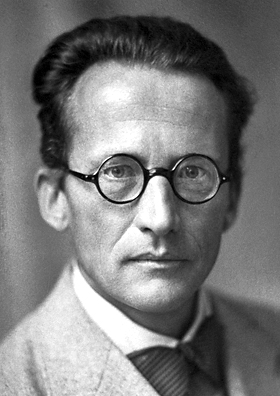
\includegraphics[width=\linewidth]{images/book3/schrodinger.jpg}
\end{minipage}\hfill
\begin{minipage}[t]{0.69\linewidth}\vspace{0pt}
{\small إرفين شرودنغر، الذي كتب سنة 1926 المعادلة الموجية التي تكون
حلولها لذرة الهيدروجين مدارات هذا الفصل، واستعاد
منها مستويات الطاقة التي كان بور قد افترضها. وتقاسم جائزة نوبل
في الفيزياء سنة 1933. (صورة: مؤسسة نوبل، ملكية عامة،
ويكيميديا كومنز.)}
\end{minipage}
\end{omfigure}

\section{الجزء الشعاعي}

احتمال وجود الإلكترون بين الكرتين اللتين نصفا قطريهما $r$ و$r +
dr$ هو $|\psi|^2$ مكاملًا على القشرة التي حجمها $4\pi r^2\,dr$؛ ومن أجل أي
مدار، بعد المكاملة على الزوايا، يساوي $r^2R^2\,dr$.

\begin{definition}[التوزيع الشعاعي]\label{def:b2:atomic-orbitals:radial-distribution}
\emph{دالة التوزيع الشعاعي}\index{دالة التوزيع الشعاعي}
لمدار هي $P(r) = r^2R_{nl}(r)^2$: فالمقدار $P(r)\,dr$ احتمال أن يقع
الإلكترون بين $r$ و$r + dr$ من النواة. و\emph{نصف القطر الأكثر
احتمالًا}\index{نصف القطر الأكثر احتمالًا} هو قيمة $r$ عند أكبر قيمة عظمى لها.
\end{definition}

\begin{proposition}[تنظيم المدار 1s]\label{prop:b2:atomic-orbitals:normalised}
$\int_0^\infty P_{1s}(r)\,dr = 1$.
\end{proposition}

\begin{proof}
مع $Z = 1$ و$r$ بوحدة $a_0$، يكون $P_{1s} = 4r^2\mathrm e^{-2r}$. وبالمكاملة بالتجزئة مرتين،
$\int_0^\infty r^2\mathrm e^{-2r}\,dr = \frac22\int_0^\infty r\,\mathrm e^{-2r}\,dr =
\frac12\int_0^\infty\mathrm e^{-2r}\,dr = \frac14$، و$4 \times \frac14 = 1$.
\end{proof}

\begin{proposition}[نصف القطر الأكثر احتمالًا]\label{prop:b2:atomic-orbitals:most-probable}
من أجل المدار 1s يكون \omterm{def:b2:atomic-orbitals:radial-distribution}{نصف القطر الأكثر احتمالًا} $a_0/Z$. ومن أجل مدار فيه $l =
n - 1$ (1s، 2p، 3d، \dots)، يكون $n^2a_0/Z$.
\end{proposition}

\begin{proof}
من أجل $l = n - 1$ لا عقدة \omterm{def:b2:atomic-orbitals:radial-angular}{للجزء الشعاعي}: $R \propto \rho^{n-1}\mathrm e^{-\rho/n}$،
ومنه $P \propto \rho^{2n}\mathrm e^{-2\rho/n}$ و$d\ln P/d\rho = 2n/\rho - 2/n$، المنعدم
من أجل $\rho = n^2$، أي $r = n^2a_0/Z$. ومع $n = 1$، $r = a_0/Z$.
\end{proof}

\begin{proposition}[متوسط نصف قطر 1s]\label{prop:b2:atomic-orbitals:mean-radius}
متوسط بعد إلكترون 1s عن النواة هو $\langle r\rangle = 3a_0/(2Z)$،
وهو أكبر من نصف قطره الأكثر احتمالًا.
\end{proposition}

\begin{proof}
مع $Z = 1$: $\langle r\rangle = \int_0^\infty r\,P(r)\,dr = 4\int_0^\infty r^3\mathrm e^{-2r}
\,dr = 4 \times 3!/2^4 = 3/2$. وللتوزيع ذيل طويل عند $r$ الكبيرة،
يسحب المتوسط إلى ما بعد القيمة العظمى.
\end{proof}

\begin{definition}[العُقد]\label{def:b2:atomic-orbitals:node}
\emph{السطح العُقدي}\index{سطح عقدي} لمدار سطح تنعدم عليه
\omterm{def:b2:atomic-orbitals:wavefunction}{الدالة الموجية} وتغيّر إشارتها. ويكون \emph{عقدة شعاعية}\index{عقدة شعاعية}
(كرة) حين ينعدم \omterm{def:b2:atomic-orbitals:radial-angular}{الجزء الشعاعي}، و\emph{عقدة
زاوية}\index{عقدة زاوية} (مستويًا أو مخروطًا يمر بالنواة) حين ينعدم
\omterm{def:b2:atomic-orbitals:radial-angular}{الجزء الزاوي}.
\end{definition}

\begin{proposition}[عدّ العقد]\label{prop:b2:atomic-orbitals:nodes}
للمدار $(n, l)$ عدد $n - l - 1$ من العقد الشعاعية و$l$ من العقد الزاوية، أي $n - 1$ في
المجموع.
\end{proposition}

\begin{proof}
على دوال \cref{thm:b2:atomic-orbitals:hydrogen}: ينعدم $R_{2s}$ عند
$\rho = 2$، و$R_{3s}$ عند جذري $2\rho^2 - 18\rho + 27$ ($\rho = 1.90$ و$7.10$)،
و$R_{3p}$ عند $\rho = 6$؛ ولا تنعدم $R_{1s}$ و$R_{2p}$ و$R_{3d}$. وينعدم \omterm{def:b2:atomic-orbitals:radial-angular}{الجزء الزاوي}
لمدار p على مستوٍ واحد ($z = 0$ للمدار $p_z$)، ولمدار d على مستويين
أو، من أجل $d_{z^2}$، على مخروط. والحالة العامة نقبلها.
\end{proof}

\begin{omfigure}
\begin{tikzpicture}
\begin{axis}[width=0.55\linewidth, height=6cm, xmin=0, xmax=24, ymin=0, ymax=0.58,
  axis x line=bottom, axis y line=left, xlabel={$r/a_0$}, ylabel={$P(r)$},
  tick label style={font=\small}, label style={font=\small}, title={\small \foreignlanguage{arabic}{التوزيعات الشعاعية، $Z = 1$}}]
\addplot[omThm, thick] table[x=r, y=s1] {figdata/out/bachelor-2-atomic-orbitals-a.dat};
\addplot[omDef, thick] table[x=r, y=s2] {figdata/out/bachelor-2-atomic-orbitals-a.dat};
\addplot[omDef, thick, dashed] table[x=r, y=p2] {figdata/out/bachelor-2-atomic-orbitals-a.dat};
\addplot[omProp, thick] table[x=r, y=s3] {figdata/out/bachelor-2-atomic-orbitals-a.dat};
\addplot[omProp, thick, dashed] table[x=r, y=p3] {figdata/out/bachelor-2-atomic-orbitals-a.dat};
\addplot[omProp, thick, dotted] table[x=r, y=d3] {figdata/out/bachelor-2-atomic-orbitals-a.dat};
\node[font=\scriptsize, omThm, anchor=west] at (axis cs:1.4,0.53) {1s};
\node[font=\scriptsize, omDef, anchor=south] at (axis cs:4.0,0.215) {2p};
\node[font=\scriptsize, omDef, anchor=south west] at (axis cs:6.4,0.17) {2s};
\node[font=\scriptsize, omProp, anchor=south] at (axis cs:10.5,0.12) {3d};
\node[font=\scriptsize, omProp, anchor=west] at (axis cs:17,0.085) {\babelsublr{3s, 3p}};
\end{axis}
\end{tikzpicture}\hfill
\begin{tikzpicture}
\begin{axis}[width=0.42\linewidth, height=6cm, xmin=0, xmax=20, ymin=-0.12, ymax=0.75,
  axis x line=middle, axis y line=left, xlabel={$r/a_0$}, ylabel={$R$},
  tick label style={font=\small}, label style={font=\small}, title={\small الأجزاء الشعاعية}]
\addplot[omDef, thick] table[x=r, y=R2s] {figdata/out/bachelor-2-atomic-orbitals-b.dat};
\addplot[omProp, thick] table[x=r, y=R3s] {figdata/out/bachelor-2-atomic-orbitals-b.dat};
\node[font=\scriptsize, omDef, anchor=west] at (axis cs:0.4,0.62) {$R_{2s}$};
\node[font=\scriptsize, omProp, anchor=west] at (axis cs:0.6,0.30) {$R_{3s}$};
\node[font=\scriptsize, anchor=south west] at (axis cs:3,0.15) {عقدة};
\draw[thin, ->] (axis cs:3,0.15) -- (axis cs:2.05,0.01);
\end{axis}
\end{tikzpicture}

{\small يمينًا: التوزيعات الشعاعية $P(r) = r^2R^2$ لمدارات الهيدروجين حتى
$n = 3$؛ فكلما كبر $n$ ابتعد الإلكترون، وللمدارات s قيم عظمى
داخلية صغيرة (النفاذ). يسارًا: يغيّر $R_{2s}$ و$R_{3s}$ إشارتيهما عند
عقدتيهما الشعاعيتين ($r = 2a_0$؛ و$1.90a_0$ و$7.10a_0$).}
\end{omfigure}

\begin{omfigure}
\begin{tikzpicture}
\begin{axis}[scale only axis, width=0.32\linewidth, height=0.32\linewidth,
  xmin=-6, xmax=6, ymin=-6, ymax=6, axis lines=none, title={\small 1s}]
\addplot[only marks, mark=*, mark size=0.25pt, omDef] table[x=x, y=y] {figdata/out/bachelor-2-atomic-orbitals-c-1s.dat};
\end{axis}
\end{tikzpicture}\hspace{0.12\linewidth}%
\begin{tikzpicture}
\begin{axis}[scale only axis, width=0.32\linewidth, height=0.32\linewidth,
  xmin=-14, xmax=14, ymin=-14, ymax=14, axis lines=none, title={\small 2s}]
\addplot[only marks, mark=*, mark size=0.25pt, omDef] table[x=x, y=y] {figdata/out/bachelor-2-atomic-orbitals-c-2s.dat};
\draw[densely dashed, omThm] (axis cs:0,0) circle[radius=2];
\end{axis}
\end{tikzpicture}

{\small صورتا كثافة النقاط للمدارين 1s و2s للهيدروجين في مستوٍ
يمر بالنواة: تتبع كثافة النقاط $|\psi|^2$ (معاينة
حتمية). وفي سحابة 2s حلقة فارغة، هي \omterm{def:b2:atomic-orbitals:node}{العقدة الشعاعية} عند $2a_0$ (متقطعة)؛
وعرض الإطارين 12 و28 $a_0$.}
\end{omfigure}

\section{الجزء الزاوي}

يحدد \omterm{def:b2:atomic-orbitals:radial-angular}{الجزء الزاوي} الشكل. فالمدار s كروي؛ والمدار p له فصّان
متعاكسا الإشارة على محوره، يفصل بينهما مستوٍ عقدي؛ والمدار d له
أربعة فصوص متناوبة الإشارة (أو، من أجل $d_{z^2}$، فصّان وحلقة). وإشارة
الفص لا معنى فيزيائيًا لها بذاتها --- فالدالتان $\psi$ و$-\psi$ تصفان الحالة
نفسها --- لكن الإشارات النسبية لمدارين تقرر، في الفصل التالي،
هل يتركبان في رابطة.

\begin{omfigure}
\begin{tikzpicture}[font=\small]
  \pic at (0,0) {oms={1}};
  \node[below] at (0,-0.75) {s};
  \pic at (2.0,0) {omp={1}{0}};
  \draw[->, black!55, thin] (1.0,0) -- (3.0,0) node[right, font=\tiny] {$x$};
  \node[below] at (2.0,-0.75) {$\mathrm p_x$};
  \pic at (4.2,0) {omp={1}{90}};
  \draw[->, black!55, thin] (4.2,-0.95) -- (4.2,0.95) node[above, font=\tiny] {$z$};
  \node[below] at (4.75,-0.75) {$\mathrm p_z$};
  \pic at (6.6,0) {omdxy}; \node[below] at (6.6,-1.0) {$\mathrm d_{xy}$};
  \pic at (9.0,0) {omdx2y2}; \node[below] at (9.0,-1.0) {$\mathrm d_{x^2-y^2}$};
  \pic at (11.4,0) {omdz2}; \node[below] at (11.4,-1.0) {$\mathrm d_{z^2}$};
\end{tikzpicture}

{\small مدارات ذرية حقيقية، رسم تخطيطي: تُظهر الفصوص المناطق التي يكون فيها $|\psi|$
كبيرًا، ملونةً بإشارة $\psi$ (الأزرق موجب، والبرتقالي سالب). وللمدارين
$\mathrm d_{xz}$ و$\mathrm d_{yz}$ شكل $\mathrm d_{xy}$ في
المستويين اللذين يدل عليهما اسماهما.}
\end{omfigure}

\begin{method}[رسم مدار انطلاقًا من أعداده الكمية]\label{met:b2:atomic-orbitals:draw-orbital}
\begin{enumerate}
  \item من $l$ يُعرف الشكل: s (كرة)، p (فصّان)، d (أربعة فصوص، أو فصّان
        وحلقة للمدار $d_{z^2}$)؛ ومن الدليل يُعرف الاتجاه.
  \item عدّ العقد الزاوية $l$ (مستويات تمر بالنواة) وأعطِ
        الفصوص المتجاورة إشارتين متعاكستين.
  \item عدّ العقد الشعاعية $n - l - 1$: قشور داخلية متعاكسة الإشارة داخل
        الفصوص الرئيسية (تُهمل عادة في الرسوم).
  \item عدّل المقياس بالمقدار $n^2a_0/Z$: كلما كبر $n$ كبر المدار؛ وكلما كبر $Z$ صغر.
\end{enumerate}
\end{method}

\section{الذرات المتعددة الإلكترونات}

في ذرة ذات عدة إلكترونات، يحس كل إلكترون بالنواة محجوبة بالإلكترونات
الأخرى. وتحتفظ المدارات بأشكال مدارات الهيدروجين، مع شحنة
فعلية $Z^*$ مكان $Z$، وتتعلق طاقة الطبقة الفرعية الآن بالعدد $l$ إضافة
إلى $n$: فإلكترون s، الذي لتوزيعه الشعاعي قيم عظمى داخلية قريبة من
النواة، يُحجب أقل من إلكترون p في الطبقة نفسها، وإلكترون p أقل
من إلكترون d.

\begin{definition}[قواعد سلاتر]\label{def:b2:atomic-orbitals:slater}
تقدّر \emph{قواعد سلاتر}\index{قواعد سلاتر} الشحنة النووية الفعلية
$Z^* = Z - \sigma$ التي يحس بها إلكترون. تُجمَّع الإلكترونات في
\babelsublr{(1s) (2s, 2p) (3s, 3p) (3d) (4s, 4p) (4d) (4f) (5s, 5p) \dots}؛ وثابت الحجب
$\sigma$ لإلكترون هو مجموع مساهمات الإلكترونات
الأخرى: 0.35 لكل إلكترون آخر من المجموعة نفسها (0.30 داخل 1s)؛
ومن أجل إلكترون s أو p، 0.85 لكل إلكترون من الطبقة $n - 1$ و1.00 لكل
إلكترون من الطبقات الأدنى؛ ومن أجل إلكترون d أو f، 1.00 لكل إلكترون
من المجموعات التي تحت مجموعته. والمجموعات التي فوقه لا تساهم بشيء.
\end{definition}

\begin{omfigure}
\small
\renewcommand{\arraystretch}{1.2}
\begin{tabular}{l|ccccc}
الإلكترون المدروس & المجموعة نفسها & الطبقة $n - 1$ & الطبقات الأدنى & المجموعات الأعلى \\ \hline
1s & 0.30 & --- & --- & 0 \\
\babelsublr{$n$s, $n$p} & 0.35 & 0.85 & 1.00 & 0 \\
\babelsublr{$n$d, $n$f} & 0.35 & 1.00 & 1.00 & 0 \\
\end{tabular}

\smallskip
{\small ثوابت حجب سلاتر، لكل إلكترون حاجب. والأعداد الكمية
الرئيسية الفعلية $n^* = 1, 2, 3, 3.7, 4.0, 4.2$ من أجل $n = 1$ إلى 6.}
\end{omfigure}

\begin{method}[حساب شحنة فعلية]\label{met:b2:atomic-orbitals:slater}
\begin{enumerate}
  \item اكتب التوزيع في مجموعات سلاتر، بترتيب $n$، مع s وp
        معًا وd وf على حدة.
  \item اختر الإلكترون؛ وأضف 0.35 لكل إلكترون آخر من مجموعته.
  \item أضف 0.85 (إلكترون s أو p) أو 1.00 (d أو f) لكل إلكترون من الطبقة التي
        تحتها مباشرة، و1.00 لكل إلكترون أعمق.
  \item $Z^* = Z - \sigma$.
\end{enumerate}
\end{method}

\begin{definition}[الطاقة المدارية ونصف القطر المداري]\label{def:b2:atomic-orbitals:orbital-energy}
في نموذج سلاتر، \emph{الطاقة المدارية}\index{طاقة مدارية} لإلكترون
شحنته الفعلية $Z^*$ وعدده الكمي الرئيسي الفعلي $n^*$ هي
$\varepsilon = -E_RZ^{*2}/n^{*2}$، و\emph{نصف قطره المداري}\index{نصف قطر مداري}
هو $n^{*2}a_0/Z^*$، أي \omterm{def:b2:atomic-orbitals:radial-distribution}{نصف القطر الأكثر احتمالًا} لمدار شبيه بالهيدروجين شحنته
$Z^*$.
\end{definition}

\begin{proposition}[طاقات سلاتر]\label{prop:b2:atomic-orbitals:slater-energy}
طاقة مجموعة من $k$ إلكترونًا شحنتها الفعلية $Z^*$ تساوي تقريبًا
$k\varepsilon = -kE_RZ^{*2}/n^{*2}$، والطاقة الإلكترونية الكلية للذرة
هي مجموعها على مجموعاتها.
\end{proposition}

\admitted

\begin{example}[الحديد: 4s أم 3d أولًا؟]\label{ex:b2:atomic-orbitals:iron}
توزيع الحديد $[\ce{Ar}]\,3\mathrm d^6\,4\mathrm s^2$. لإلكترون 4s: $\sigma = 0.35 + 14
\times 0.85 + 10 \times 1.00 = 22.25$، $Z^* = 3.75$، $\varepsilon = -13.6 \times
3.75^2/3.7^2 = \qty{-14.0}{eV}$. ولإلكترون 3d: $\sigma = 5 \times 0.35 + 18 \times 1.00 =
19.75$، $Z^* = 6.25$، $\varepsilon = -13.6 \times 6.25^2/9 = \qty{-59}{eV}$. فإلكترونات
3d مرتبطة بقوة أكبر بكثير: ومع أن 4s يُملأ أولًا في ترتيب
البناء، فإن إلكترون 4s هو الذي يغادر حين يتأين الحديد، وتوزيع
أيون الحديد(II) هو $[\ce{Ar}]\,3\mathrm d^6$.
\end{example}

\section{استعمال طاقات المدارات وأحجامها}

\begin{proposition}[طاقة التأين من طاقات سلاتر]\label{prop:b2:atomic-orbitals:ionisation}
في نموذج سلاتر، طاقة التأين الأولى لذرة هي الفرق
بين الطاقتين الكليتين للأيون وللذرة، المحسوبتين مجموعةً مجموعةً
بالشحنات الفعلية لكل منهما.
\end{proposition}

\begin{proof}
طاقة التأين هي $E(\text{أيون}) - E(\text{ذرة})$؛ وحسب
\cref{prop:b2:atomic-orbitals:slater-energy}، كلتاهما مجموع طاقات مجموعات، 
ولا تتغير إلا المجموعة التي تفقد الإلكترون (فالمجموعات الداخلية لا تحجبها
الإلكترونات الخارجية).
\end{proof}

\begin{example}[الكربون]\label{ex:b2:atomic-orbitals:carbon}
الكربون، \babelsublr{(2s, 2p)$^4$}: $Z^* = 6 - 2 \times 0.85 - 3 \times 0.35 = 3.25$؛ وطاقة المجموعة
$4 \times (-13.6 \times 3.25^2/4) = \qty{-143.6}{eV}$. والأيون \ce{C+}، \babelsublr{(2s, 2p)$^3$}: $Z^* =
3.60$، $3 \times (-13.6 \times 3.60^2/4) = \qty{-132.2}{eV}$. فطاقة التأين
\qty{11.5}{eV}، مقابل \qty{11.26}{eV} مقيسة.
% ledger: ie:C, const:RyhcEV
\end{example}

\begin{omfigure}
\begin{tikzpicture}
\begin{axis}[width=0.47\linewidth, height=5.4cm, xmin=0.5, xmax=8.5, ymin=0, ymax=6.5,
  axis x line=bottom, axis y line=left, xtick={1,2,3,4,5,6,7,8},
  xticklabels={Li,Be,B,C,N,O,F,Ne}, tick label style={font=\small},
  label style={font=\small}, title={\small الدورة 2}]
\addplot[omThm, thick, mark=*, mark size=1.3pt] table[x=k, y=zs] {figdata/out/bachelor-2-atomic-orbitals-d-period.dat};
\addplot[omDef, thick, mark=square*, mark size=1.3pt] table[x=k, y=r] {figdata/out/bachelor-2-atomic-orbitals-d-period.dat};
\node[font=\scriptsize, omThm, anchor=south east] at (axis cs:7.8,5.3) {$Z^*$};
\node[font=\scriptsize, omDef, anchor=south west] at (axis cs:1.2,3.1) {\shortstack{\foreignlanguage{arabic}{نصف القطر ($a_0$)}}};
\end{axis}
\end{tikzpicture}\hfill
\begin{tikzpicture}
\begin{axis}[width=0.47\linewidth, height=5.4cm, xmin=1.5, xmax=6.5, ymin=0, ymax=9,
  axis x line=bottom, axis y line=left, xtick={2,3,4,5,6},
  xticklabels={Li,Na,K,Rb,Cs}, tick label style={font=\small},
  label style={font=\small}, title={\small الزمرة 1}]
\addplot[omThm, thick, mark=*, mark size=1.3pt] table[x=n, y=zs] {figdata/out/bachelor-2-atomic-orbitals-d-group.dat};
\addplot[omDef, thick, mark=square*, mark size=1.3pt] table[x=n, y=r] {figdata/out/bachelor-2-atomic-orbitals-d-group.dat};
\node[font=\scriptsize, omThm, anchor=north] at (axis cs:4,2.0) {$Z^*$};
\node[font=\scriptsize, omDef, anchor=west] at (axis cs:2.1,5.4) {\shortstack{\foreignlanguage{arabic}{نصف القطر ($a_0$)}}};
\end{axis}
\end{tikzpicture}

{\small شحنة سلاتر الفعلية لإلكترون التكافؤ \omterm{def:b2:atomic-orbitals:orbital-energy}{ونصف القطر المداري}
$n^{*2}a_0/Z^*$. على طول الدورة 2، تزداد $Z^*$ بمقدار 0.65 لكل عنصر وتنكمش
الذرات؛ ونزولًا في الزمرة 1، تبقى $Z^*$ عند 1.30 ثم 2.20 بينما يكبر $n^*$، فتنتفخ
الذرات.}
\end{omfigure}

يعيد النموذج إنتاج اتجاهات مجلد السنة الأولى. فعلى طول الدورة يُحجب كل
بروتون مضاف بمقدار 0.35 فقط من الإلكترون المضاف معه: فترتفع $Z^*$،
وينكمش المدار الخارجي ويرتبط بقوة أكبر. ونزولًا في الزمرة، لا تكاد $Z^*$
تتغير بينما تبتعد الطبقة الخارجية: فتكبر الذرات وتنخفض طاقات تأينها.
والصوديوم، مع $Z^* = 2.20$ لإلكترونه 3s، \omterm{def:b2:atomic-orbitals:orbital-energy}{نصف قطره المداري}
$9/2.2 = 4.1a_0$؛ والكلور، مع $Z^* = 6.10$ لإلكترون 3p، $9/6.1 = 1.5a_0$.

\section{تمارين}

\begin{exercise}[$\star$]\label{exo:b2:atomic-orbitals:1}
أعطِ العددين الكميين $n$ و$l$، وعدد العقد الشعاعية والعقد الزاوية
لمدار 3p ولمدار 4d.
\end{exercise}

\begin{exercise}[$\star$]\label{exo:b2:atomic-orbitals:2}
بيّن انطلاقًا من $R_{2p}$ أن \omterm{def:b2:atomic-orbitals:radial-distribution}{نصف القطر الأكثر احتمالًا} لإلكترون 2p في الهيدروجين
هو $4a_0$، وأعطه بالبيكومتر.
\end{exercise}

\begin{exercise}[$\star$]\label{exo:b2:atomic-orbitals:3}
احسب احتمال وجود إلكترون 1s في الهيدروجين أقرب إلى
النواة من $a_0$.
\end{exercise}

\begin{exercise}[$\star$]\label{exo:b2:atomic-orbitals:4}
ارسم بخطوط تقريبية المدار $3\mathrm d_{xy}$: الفصوص، والإشارات، والمستويات العقدية. وكم
\omterm{def:b2:atomic-orbitals:node}{عقدة شعاعية} له؟
\end{exercise}

\begin{exercise}[$\star\star$]\label{exo:b2:atomic-orbitals:5}
احسب شحنة سلاتر الفعلية لإلكترون 2p في الأكسجين \omterm{def:b2:atomic-orbitals:orbital-energy}{ونصف القطر
المداري} الذي تعطيه.
\end{exercise}

\begin{exercise}[$\star\star$]\label{exo:b2:atomic-orbitals:6}
مستعملًا مثال الحديد، فسّر لماذا يكون توزيع \ce{Fe^3+}
$[\ce{Ar}]\,3\mathrm d^5$ وليس $[\ce{Ar}]\,3\mathrm d^3 4\mathrm s^2$.
\end{exercise}

\begin{exercise}[$\star\star$]\label{exo:b2:atomic-orbitals:7}
قدّر \omterm{def:b2:atomic-orbitals:slater}{بقواعد سلاتر} طاقتي التأين الأوليين لليثيوم والصوديوم،
وقارن بالقيمتين المقيستين 5.39 و\qty{5.14}{eV}. وعلّق.
\end{exercise}

\begin{exercise}[$\star\star$]\label{exo:b2:atomic-orbitals:8}
احسب $Z^*$ \omterm{def:b2:atomic-orbitals:orbital-energy}{ونصف القطر المداري} للإلكترون الخارجي للصوديوم
وللكلور، وفسّر لماذا تكون ذرة الصوديوم أكبر.
\end{exercise}

\begin{exercise}[$\star\star$]\label{exo:b2:atomic-orbitals:9}
بيّن أن المدارين 1s و2s للهيدروجين متعامدان،
$\int\psi_{1s}\psi_{2s}\,dV = 0$.
\end{exercise}

\begin{exercise}[$\star\star\star$]\label{exo:b2:atomic-orbitals:10}
اكتب $R_{2p} = N\rho\,\mathrm e^{-\rho/2}$ وأوجد الثابت $N$ الذي ينظّمه
($Z = 1$، و$r$ بوحدة $a_0$).
\end{exercise}

\begin{exercise}[$\star\star\star$]\label{exo:b2:atomic-orbitals:11}
قارن متوسط نصف القطر \omterm{def:b2:atomic-orbitals:radial-distribution}{ونصف القطر الأكثر احتمالًا} لإلكترون 1s، 
وفسّر انطلاقًا من شكل $P(r)$ لماذا يختلفان.
\end{exercise}

\begin{exercise}[$\star\star\star$]\label{exo:b2:atomic-orbitals:12}
أوجد \omterm{def:b2:atomic-orbitals:node}{السطح العقدي} للمدار $\mathrm p_z$ وبيّن أن $\psi_{2p_z}$
تغيّر إشارتها عبره. وما \omterm{def:b2:atomic-orbitals:wavefunction}{كثافة الاحتمال} على هذا السطح؟
\end{exercise}

\section{مسألة: أين الإلكترون؟}

\begin{problem}[{مسألة نهاية الأسبوع --- المدار 1s للهيدروجين وأنصاف أقطاره،
واحتمال وجود الإلكترون أبعد من مسافة معيّنة، وعُقد المدارين 2s و2p
وقيمهما العظمى، وتقدير سلاتر لطاقات تأين الكربون
والنيتروجين والأكسجين}]
\label{pb:b2:atomic-orbitals:1}
المعطيات: $a_0 = \qty{52.9}{pm}$؛ $E_R = \qty{13.6}{eV}$؛ وطاقات التأين الأولى المقيسة
(\unit{eV}): C 11.26، N 14.53، O 13.62. $\psi_{1s} = \pi^{-1/2}a_0^{-3/2}\,
\mathrm e^{-r/a_0}$.
% ledger: const:a0, const:RyhcEV, ie:C, ie:N, ie:O

\medskip
\noindent\textbf{الجزء الأول --- المدار 1s.}
\begin{enumerate}
  \item تحقق من أن $\psi_{1s}$ منظَّمة، مستعملًا $dV = 4\pi r^2\,dr$.
  \item اكتب \omterm{def:b2:atomic-orbitals:radial-distribution}{دالة التوزيع الشعاعي} $P(r)$.
  \item أوجد \omterm{def:b2:atomic-orbitals:radial-distribution}{نصف القطر الأكثر احتمالًا}.
  \item احسب متوسط نصف القطر.
  \item لماذا يكون المتوسط أكبر من \omterm{def:b2:atomic-orbitals:radial-distribution}{نصف القطر الأكثر احتمالًا}؟
  \item \omterm{def:b2:atomic-orbitals:wavefunction}{كثافة الاحتمال} أكبر ما يمكن عند النواة، ومع ذلك $P(0) = 0$.
        فسّر.
  \item أعطِ \omterm{def:b2:atomic-orbitals:radial-distribution}{نصف القطر الأكثر احتمالًا} بالبيكومتر.
\end{enumerate}

\medskip
\noindent\textbf{الجزء الثاني --- أبعد من نصف قطر.}
\begin{enumerate}[resume]
  \item بيّن أن احتمال وجود الإلكترون أبعد من $r_0 =
        xa_0$ هو $\mathrm e^{-2x}(1 + 2x + 2x^2)$.
  \item احسبه من أجل $r_0 = a_0$.
  \item احسبه من أجل $r_0 = 2a_0$.
  \item أوجد بالتجربة والخطأ نصف قطر الكرة التي تحوي الإلكترون
        باحتمال قدره 0.90.
  \item بأي معنى لا حافة للذرة، وبأي معنى لها حجم؟
\end{enumerate}

\medskip
\noindent\textbf{الجزء الثالث --- 2s و2p.}
\begin{enumerate}[resume]
  \item أعطِ عقد 2s و2p (عددها، ونوعها، وموقعها).
  \item أين يغيّر $R_{2s}$ إشارته؟
  \item أوجد \omterm{def:b2:atomic-orbitals:radial-distribution}{نصف القطر الأكثر احتمالًا} للمدار 2p.
  \item أوجد القيمتين العظميين للدالة $P_{2s} \propto r^2(2 - r)^2\mathrm e^{-r}$ ($r$ بوحدة
        $a_0$).
  \item أي المدارين 2s و2p له كثافة إلكترونية أقرب إلى النواة؟ وماذا
        يعني ذلك في ذرة متعددة الإلكترونات؟
  \item كيف تتغير أنصاف الأقطار هذه في الأيون الشبيه بالهيدروجين \ce{C^5+}؟
\end{enumerate}

\medskip
\noindent\textbf{الجزء الرابع --- الكربون والنيتروجين والأكسجين.}
\begin{enumerate}[resume]
  \item احسب شحنة سلاتر الفعلية $Z^*$ لإلكترون 2p في C وN وO.
  \item احسب الطاقات المدارية الموافقة.
  \item قدّر طاقة التأين الأولى للكربون بوصفها فرقًا بين طاقات
        مجموعات.
  \item والسؤال نفسه للنيتروجين.
  \item والسؤال نفسه للأكسجين، وقارن القيم الثلاث بالقيم المقيسة.
  \item أي سمة من سمات القيم المقيسة يفوّتها النموذج، ولماذا؟
  \item اذكر احتمال وجود إلكترون 1s في الهيدروجين أبعد
        من $2a_0$.
\end{enumerate}
\end{problem}
